'\documentclass[sigconf, anonymous]{acmart}

\fancyhf{} % Remove fancy page headers 
\fancyhead[C]{Anonymous submission \#9999 to ACM CCS 2018} % TODO: replace 9999 with your paper number
\fancyfoot[C]{\thepage}

\setcopyright{none} % No copyright notice required for submissions
\acmConference[Anonymous Submission to ACM CCS 2018]{ACM Conference on Computer and Communications Security}{Due 19 May 2018}{Toronto, Canada}
\acmYear{2018}

\settopmatter{printacmref=false, printccs=true, printfolios=true} % We want page numbers on submissions
\usepackage{subcaption}
%%\ccsPaper{9999} % TODO: replace with your paper number once obtained

\begin{document}

\title{Template for ACM CCS 2018} % TODO: replace with your title

\begin{abstract}
Your abstract should go here. You will also need to upload a plain-text abstract into the web submission form.
\end{abstract}

% TODO: replace this section with code generated by the tool at https://dl.acm.org/ccs.cfm
\begin{CCSXML}
<ccs2012>
<concept>
<concept_id>10002978.10003029.10011703</concept_id>
<concept_desc>Security and privacy~Usability in security and privacy</concept_desc>
<concept_significance>500</concept_significance>
</concept>
</ccs2012>
\end{CCSXML}

\ccsdesc{Security and privacy~Use https://dl.acm.org/ccs.cfm to generate actual concepts section for your paper}
% -- end of section to replace with generated code

\keywords{template; formatting; pickling} % TODO: replace with your keywords

\maketitle

\section{Introduction}
\label{sec:introduction}

\section{Background}
\label{sec:background}

\section{Related Work}
\label{sec:related_work}

\section{MoneTor design}
\label{sec:design}
Where we previously assumed the existence of an ideal payment procedure, we now
describe our construction for the MoneTor payment scheme. We first summarize the
algorithmic design of our payment protocols and proceed to describe integration
details with the Tor networking layer and codebase.

\subsection{Security Model}

The privacy threat model is derived from the local active adversary
model ubiquitously found in Tor research~\cite{dingledine2004tor}. Informally, we claim the following
anonymity guarantees:

\begin{enumerate}
\item No additional party needed to operate the MoneTor system (i.e. ledgers
  and intermediaries) will know any more about a given user than would be known
  by an additional middle relay.
\item In typical usage, users do not leak any more information other than the
  single bit needed to differentiate premium and nonpremium users.
\end{enumerate}

Our threat model for payment security is similar to those found in prior works
in blockchain micropayment channels~\cite{poon2016bitcoin}. In such models, the
user is protected from malicious intermediaries by the ability to prove
misbehavior to a global ledger. The security guarantees on the ledger will be
subject to the guarantees made by the cryptocurrency
interface~\cite{back2014enabling, poon2017plasma}. This is in direct contrast to
prior to Chaumian e-cash proposals that employ an \emph{honest but curious}
model for the central bank. In MoneTor, we prioritize payment security and
ensure that nobody, including the ledger, ever has direct control of user funds.

\subsection{Payment Protocols}

In this section we specify formal protocols that comprise the payment
scheme. All protocols are either two or three party interactions between a
subset of the following roles: $C$ (client), $R$ (relay), $E$ (end user: either
a client or relay) $I$ (intermediary), and $L$ (ledger). At this level, we
assume that one client is paying one relay through a single channel and that
network-layer anonymity will be sufficiently handled at the Tor protocol level.

The full MoneTor payment scheme is a superset of Bolt three-party bidirectional
micropayment channels and, as such, we adopt its nomenclature where possible but
adapt it to our notions of ledgers, clients, relays, etc. The following is brief
outline of the prerequisite micropayment channel procedures defined in Bolt. We
refer the reader to the original paper for more detailed
specifications~\cite{green2017bolt}.

\begin{itemize}
\item $KeyGen$: Any party generates a cryptographic keypair
\item $Init_E$: $E$ initializes her half of a micropayment channel by escrowing
  initial funds on $L$
\item $Init_I$: $I$ initializes his half of a micropayment channel by
  escrowing intial funds on $L$
\item $Establish$: $E$ and $I$ interact to establish a new, functional
  micropayment channel
\item $Pay$: $E_1$ interacts with $I$ and $E_2$ to send a single micropayment to $E_2$
\item $Refund$: $E$ closes a micropayment channel on $L$ and makes a claim on
  the escrowed balance.
\item $Refute$: $I$ closes a micropayment channel on $L$ and makes a claim on
  the escrowed balance.
\item $Resolve$: $L$ determines the final balance of funds awared to
  each party.
\end{itemize}

While anonymous micropayment channels present a tremendous advance for many
applications, the relatively heavy cryptography ($37-100 ms$) and communication
(7 message legs) are a prohibitive expense for Tor relay payment. In addition to
concerns regarding global network overhead, it is also desirable to keep the
barrior threshold low for small perspective relay operators. We therefore
introduce a new payment layer that enables the first practically efficient
payments for Tor routing.

MoneTor makes use of the existing anonoymous micropayment structure to
facilitate \emph{locally transparent nanopayments}. In this scheme,
\emph{nanopayment channels} are established in place of a single micropayment
operation. Nanopayment channels allow the client to send a $n$ number of
undirectional nanopayments to the relay. Each payment represents a fixed value
$\delta$, established at the start of the nanopayment channel. The payments
themselves are \emph{locally transparent} in the sense that each nanopayment in
the same channel is trivially linked to each other. However, each nanopayment
channel is anonymous with respect to other nanopayment channels and micropayment
operations.

Assuming that $C$ and $R$ have both completed $Establish$ with $I$, we define
the following set of protocols needed to operate a nanopayment channel.

\begin{itemize}
\item $Nano$-$Setup$: $C$ and $I$ interact to prepare a nanopayment channel on top
  of their existing micropayment channel.
\item $Nano$-$Establish$: $C$ sends her nanopayment channel information to $R$,
  who establishes it with $I$ on top of their existing micropayment channel.
\item $Nano$-$Pay$: $C$ sends a single nanopayment channel to $R$. This is
  repeatable for up to $n$ operations.
\item $Nano$-$Close_R$: $R$ closes his nanopayment channel with $I$.
\item $Nano$-$Close_C$: $C$ closes his nanopayment channel with $I$. Note that
  this must happen after $Nano$-$Close_R$.
\end{itemize}

We also specify the following modified channel conflict resolution procedures to
ensure secure closure properties for the nanopayment scheme.

\begin{itemize}
\item $Nano$-$Refund$: $E$ closes channel on $L$.
\item $Nano$-$Refute$: $I$ closes channelon $L$.
\item $Nano$-$Resolve$: $L$ makes final determination on both micropayment and
  outstanding nanopayment balances.
\end{itemize}

The core of our nanopayment scheme is inspired by the classic \emph{Payword}
two-party micropayment scheme in which payments are encoded by successively
revealed preimages in a precomputed hash chain~\cite{rivest1996payword}. Hash
chains are perhaps the most efficient known method for representing payments. In
contrast to the expensive zero-knowledge proofs and signatures involved in
anonymous micropayments, a single payment can be computed in the order of
millions per second and conferred with a 256 bit message, or one single Tor
cell.

The challenge in this construction is to securely integrate the hash chain
concept into the existing three-party anonymous micropayment channel setup such
that all parties maintain cryptographic ownership of their funds. At the same
time, we must ensure that no deanonymizing information is leaked outside of the
nanopayment channel context. The scheme we present incurrs an overhead penalty
of approximately one micropayment operation at the beginning and end of each
nanopayment channel lifecyle.

\subsection{Nanopayment Protocols}
tio
In this section, we provide a summarized intuition for the basic steps in the
payment protocol. For a more formal algorithmic definition, we refer the reader
to [algorithms] and [Appendix].

\textbf{Nano-Setup} At the start of this protocol, $C$ has access to a
micropayment wallet $w$ that enables her to operate her micropayment channel
with $I$ as well as a refund token $rt$ that entitles her to claim her current
funds on $L$ should $I$ misbehave or go offline. To construct a nanopayment
channel, $C$ first generates an array of values $hc$ of length $n$ where
$hc_i = H(hc_{i+1})$ and $hc_n$ is a random number. The root of the hash chain
$hc_0$ is used to create a globally unique nanopayment token $nT$ that encodes
the public parameters of the nanopayment channel including the length $n$ and
the per-payment value $\delta$. $C$ sends $I$ a commitment to a fresh
nanopayment channel parametrized by $nT$ along with a zero-knowledge proof of
the following statements:

\begin{enumerate}
\item The nanopayment wallet $nw$ is well-formed from $w$
\item $C$ has ownership of a micropayment channel containing at least $n *
  \delta$ funds.
\end{enumerate}

$I$ verifies these messages and blindly supplies $C$ with a new refund token $nrt$
that entitles $C$ to cash out the full balance of the micropayment channel along
with any nanopayments to $L$. $C$, now protected against misbehavior by $I$,
agrees to send a revocation token $\sigma_w$, which revokes her right to use $w$
or $rt$. $I$, now protected against double spending by $C$, can now safely
inform $C$ that the nanopayment channel has been setup.

\textbf{Nano-Establish} At this point, $C$ sends $R$ the same $nT$ token used to
setup the channel with $I$. $R$ uses this token to initiate her end of the
nanopayment channel with $I$ with essentially the same procedure that $C$ used
in $Nano$-$Setup$. The nanopayment channel is fully established and ready to be
used. A key observation is that both ends of the channel ($C$-$I$ and $R$-$I$)
are rooted at the same hash chain root $hc_0$. As a result, the scheme ensures a
correct-by-construction notion of \emph{atomicity} whereby both legs of the
protocol are complete at the same time.

\textbf{Nano-Pay} To make the next payment $i$, $C$ simply sends the next hash preimage $hc_i$ to
$R$. Knowledge of this preimage $hc_i$ is sufficient for $R$ to prove posession
of a nanopayment. At any given time, $R$ can broadcast the tuple ($nrt$, $hc_i$)
to $L$ to prove ownership of a certain value of funds. Notice that this action
simultaneously reveals $hc_i$ to $I$, who can then claim an equivalent value of
funds from $C$.

\textbf{Nano-Close} After some number of payments $k < n$ has transpired, $C$ and $R$ will both wish
to close their nanopayment channels through $I$. In this process, the $R$-$I$ leg
must be closed before the $C$-$I$ leg. This is due to the unidirectional nature
of nanopayment channels. Since payments are flowing form $C$ to $R$, $I$ must
first determine its debt to $R$ in order to know how much it can claim from $C$.

$R$ first sends to $I$ a commitment to a new micropayment wallet $w'$ and a
zero-knowledge proof of the following statements:

\begin{enumerate}
\item $w'$ is well-formed from $w$
\item The balance of $w'$ is equal to the sum of the previous wallet $w$ and
  $\delta * k$
\end{enumerate}

Once verified, $I$ issues a refund token $rt'$ on the new funds. $R$ agrees to
invalidate the nanopayment channel by issuing a revocation token $\sigma_{nw}$
to $I$. $I$ and $R$ proceed to create a blind signature on $w'$ thus validating
the wallet for future use.

Once $I$ has closed his nanopayment channel leg with $R$, $I$ and $C$ are free
to complete the exact same close protocol. All parties are now reverted to the
original state prior to $Nano$-$Setup$ with a securely updated balance.

\subsection{Network Protocols}
%needs an overview of the protocol extension and some nicelydone image
%some theoretical discussion about how to properly anonymize R->I, C->I, R/C->L connections using Tor circuits. 
%memory cost/cpu cost discussion
\subsection{Implementation}


\section{Experimental Analysis}
\label{sec:analysis}
%\op{Is it only validation? It seems that some of the paramters are also chosen based on these simulations. Also, the discussion seems to be using some parameters which are only made explicit later. For instance, in 7.1.2, the circuits with less than 1000 cells are described as useless for premium. The reson for that seems to only become clear when reading 8.3.1, which indicates that payments are made after 1000 cells. I wonder if, at the end of this section, and before the experimental analysis, it would make sense to add a frame that sums-up what protocol will be analyzed, including the parameters: what channels and circuits are created when, when is payment happening, when are channels closed, \dots}

\subsection{Data Collection}
\label{subsec:datacollection}

We deployed during two weeks a data collection system to look for empirical temporal information
about lifetime and bandwidth consumption in Tor circuits. Our objective was to
have a deeper understanding of typical Tor usage and whether such usage can
benefit from our channel-based payment system. For example, these measurements
might capture some notion about the type and magnitude of potential premium
traffic. We classify the traffic type based on the service connection
port. Besides the classical ports 80 and 443 used for web traffic, we aggregate
data from some other families including the WHOIS
protocol~\cite{daigle2004whois} and RWHOIS~\cite{williamson1994referral} from
ports 43 and 4321, respectively. The complete list of families is constructed
from the reduced exit policies which we run on our relays. This measurement
methodology allows us to reason based on application specific traffic.

% We interested to know about the distribution lifetime of Tor circuits for each
% port we allow. We are also interested to picture how many cells those circuits
% handled through their lifetime with some level of granularity.

\subsubsection{Efforts to preserve users privacy}

To ensure ethical experimentation, we first contacted the Tor research safety
board~\cite{torsafety}. The feedback we received was subsequently used to refactor our data
collection process (e.g., no metadata from any specific flow or circuit should be written on disk).

Data from five old and very stable exit relays with a total bandwidth of 50 MiB/s was collected, stripped of
origin metadata, and aggregated on a central server. The data collected from each
relay is itself an aggregation which we perform inside the relay's memory. The aggregation is done only for ``active circuits'' from the exit relay perspective. We consider a circuit active when it has received a connection request to an IP address on the internet.
%The data collection is probabilistic; only 30\% of the circuits processed by our
%relays were considered in order to maintain plausible deniability on the
%clients' behalf.
The aggregation is done inside bins of configurable size for
every different traffic family we consider. Once we collected enough data from a
single family, we dump the information on the disk, clear the data, and resume a
new session. The final information obtained contains an aggregation of 1600
circuits over an unspecified time frame that is implicitly determined by the
rate of user activity. The following data was considered:

\begin{itemize}
\item \textbf{Time Profile}: The number of cells in each time interval
  (configured to be 5 seconds) since the success of the DNS request. This
  information sums inbound and outbound cells, and is aggregated over circuits
  by addition.
\item \textbf{Total Counts}: The total amount of cells processed by a
  circuit. This information is aggregated by taking the mean of fixed-size
  nearest neighbor bins.
\end{itemize}

Crucially, we do not record information linked to any single particular user
flow on disk.
%The code used for the data collection will be made available for
%audit online.

\subsubsection{Observations}

\begin{figure} \centering
  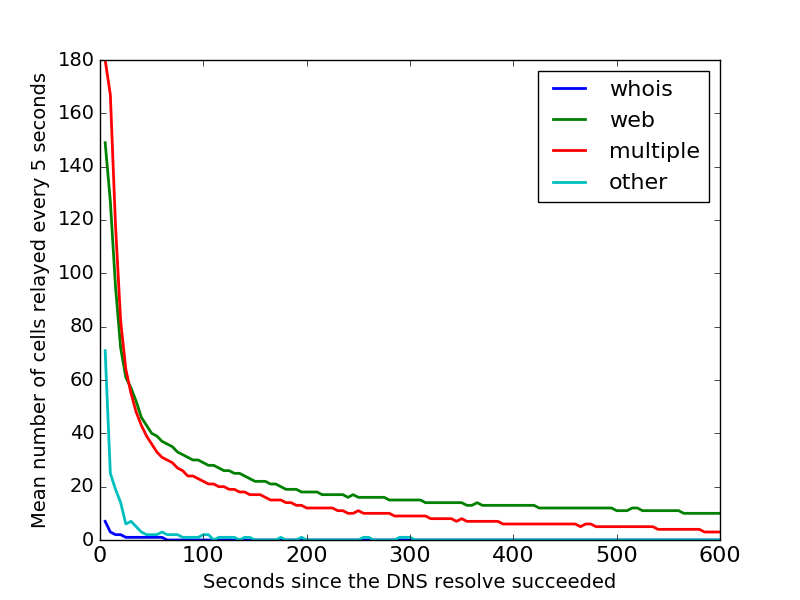
\includegraphics[width=0.4\textwidth]{images/exitmeasurement.png}
  \caption{Time Profile --- Average distribution of traffic across circuit
    lifetime beginning with the first DNS request.}
  \label{fig:statsa}
\end{figure}
\begin{figure} \centering
  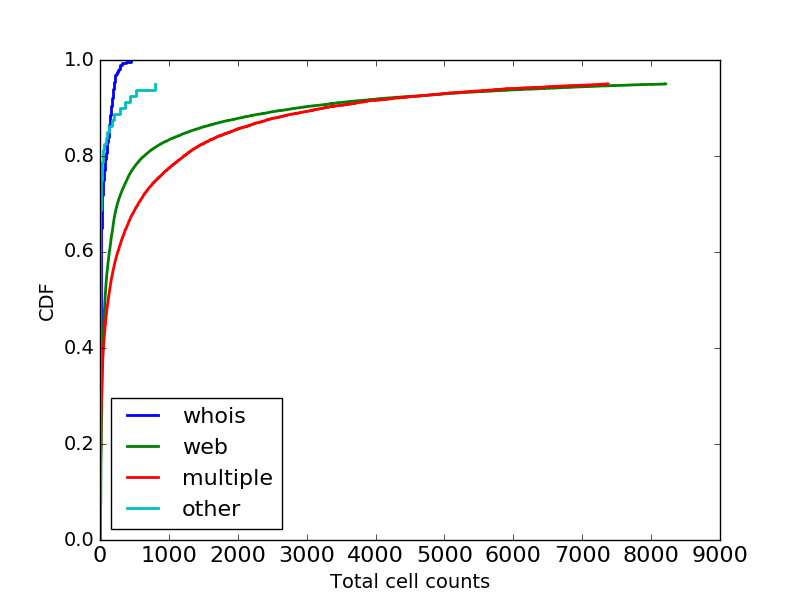
\includegraphics[width=0.4\textwidth]{images/totcellcountscdf.png}
  \caption{Total Counts --- Distribution of circuit size with respect to the
    total number of cells processed}
\label{fig:statsb}
\end{figure}


Our measurements successfully captured several important pieces of information
for the design and justification of moneTor. For example, one important task is
to determine the number of potential users that could benefit from paid
traffic. From Figure~\ref{fig:statsb}, we observe that $\approx 82\%$ of
circuits carrying only web traffic exchanged less than 1000 cells. While we
cannot deduce any statements about users, we can speak to the fraction of
circuits that may benefit from a payment channel in the Tor network, since
around $50\%$ of them do not carry data and less than $17\%$ of them carry at
least one web page. The remaining $18\%$ would appear to be better candidates
for moneTor.

It is also evident from Figure~\ref{fig:statsa} that most of the traffic is usually
carried within the first few tens of seconds, and that all types of traffic we
collected seems to follow the same rule. From that result, we believe that the
reliability of payment is critical within the first few seconds, especially from
a relay viewpoint. Our payment channels should ideally be established and ready
before the user begins to use the circuit. While this result cannot be
guaranteed for an unbounded number of circuits, a well-designed preemptive
circuit build strategy should do a sufficient job of eliminating channel
setup/establish latency in the average case.

%% In another area of research, it may be interesting to point out that since %
%$\approx 50\%$ of users do not carry data after their DNS request, some %
%adversary doing end-to-end correlation may prefer to use active attacks over %
%passive correlation to capture more identities.

\section{Simulated Validation}
\label{sec:experimentations}

Having established the empirical context for a channel payment scheme, we
validated our technical design via experiments performed on a prototype
software implementation within the native Tor codebase.

\subsection{Prototype}

A substantial contribution of the research is embedded within our implementation
of the moneTor framework. The modifications, applied to Tor release version
0.3.2.10, cover approximately fifteen thousand added lines of code across Tor's
core C software. We emphasize that the implementation is not a fully functional
prototype and is optimized solely for our experiments. Most notably, we
simulated crytographic operations in the nanopayment creation and close
procedures using CPU delays. These delays were tuned to conservatively reflect
real measurements in background work~\cite{green2017bolt}.\footnote{Extracted
  values are conservative in the sense that our zero-knowledge proofs require
  proving only a subset of the statements required in each corresponding Bolt
  zero-knowledge proof.} The partial prototype serves the following purposes in
our study.

\begin{enumerate}
\item An implementation covering nuances not explicitly
  covered in the protocol designs. In effect, we would like to show that there
  are no unexpected and prohibitive practical conflicts with the existing Tor
  design.
\item A platform to study the feasibility of premium circuit
  prioritization from a networking perspective.
\item A platform to obtain a rough factor-of-two approximation for all
  bandwidth, computation, and memory requirements of the system, both globally
  and at individual nodes.
\end{enumerate}

The first design purpose is clearly qualitative and we briefly note that we did
not discover any insurmountable logical flaws in the design. To analyze the
networking dynamics and resource consumption, we studied our implementations
through the following proceeding experiments.

\subsection{Methodology}
\label{subsec:methodology}

Experiments were conducted using the Tor shadow simulator
tool~\cite{jansen2011shadow}. We ran two sets of experiments at different
scales from a consensus document published in early February 2018. The first set featured 100 relays, 1000 clients, 10 intermediaries, and
ran for a total of 90 minutes. These experiments were used to gather information
concerning the system overhead and protocol execution times. The second set
featured 250 relays, 2500 clients, 25 intermediaries, 80 minutes of total run
time, and was used to measure the performance benefits conferred to premium
clients. In both cases, simulated traffic features 16\% \emph{bulk} clients who
continuously download 5 MiB files and 84\% \emph{web} clients who periodically
download 2 MiB files,\footnote{While 5 MiB bulk files are a common standard in
  Tor benchmarking~\cite{portal2018tormetrics}, 2 MiB web files reflect the
  approximate size of modern web pages~\cite{team2018httparchive}}. The number
and behavior of clients were chosen to satisfy (A) realistic congestion rates
measured by a transfer timeout percentage around 4\%~\cite{portal2018tormetrics}
and a historical bulk/web global traffic ratio of about
50\%~\cite{chaabane2010digging, mccoy2008shining}. Importantly, it should be
noted that neither the scale of our experiments nor the precise configuration of
client nodes are intended to be precise replicas of real-world conditions. Tor
networking is itself a complex area of research and we are content to adopt the
simplest model that will highlight the relatively crude networking needs of our
incentivization scheme.

\subsection{Experiments}
\label{subsec:experiments}
Our experiments are separated into three groups each capturing a separate
characteristic of the scheme.

\subsubsection{Global Overhead}

First, we attempt to show the total cost the moneTor scheme in terms of total
network throughput. To highlight worst-case performance, we configured a medium
scale experiment consisting of 100\% of premium clients and compare to a
baseline trial with 0\% premium clients. No actual traffic priority is
conferred. Since our algorithms makes use of some concurrent crytpographic
operations, we are concerned with the number of CPU cores available to most
relays. This information is not publicly available. As a result, we 
provide two trials with moneTor: one where we assume all nodes are running on
multi-core hardware and one in which all nodes are running on single-core
hardware. The results are summarized in Figure~\ref{fig:overhead}.

% Add information about how we simulate singlecore and multicore hardware
% That gonna overflow 12 pages, though :/

\begin{figure*} \centering
	\begin{subfigure}[t]{0.32\textwidth} \centering
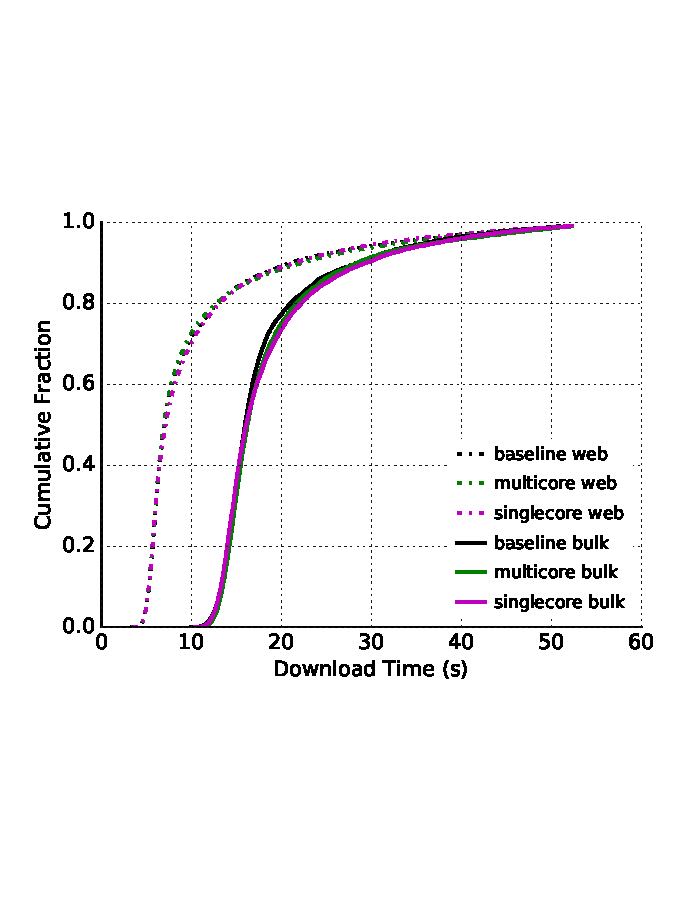
\includegraphics[trim={0 3cm 0 3cm}, clip, width=1.0\textwidth]{images/overhead_downloadtime.pdf}
		\caption{Download Time Overhead}
		\label{fig:overhead_ttlastbyte}
	\end{subfigure}
	\begin{subfigure}[t]{0.32\textwidth} \centering
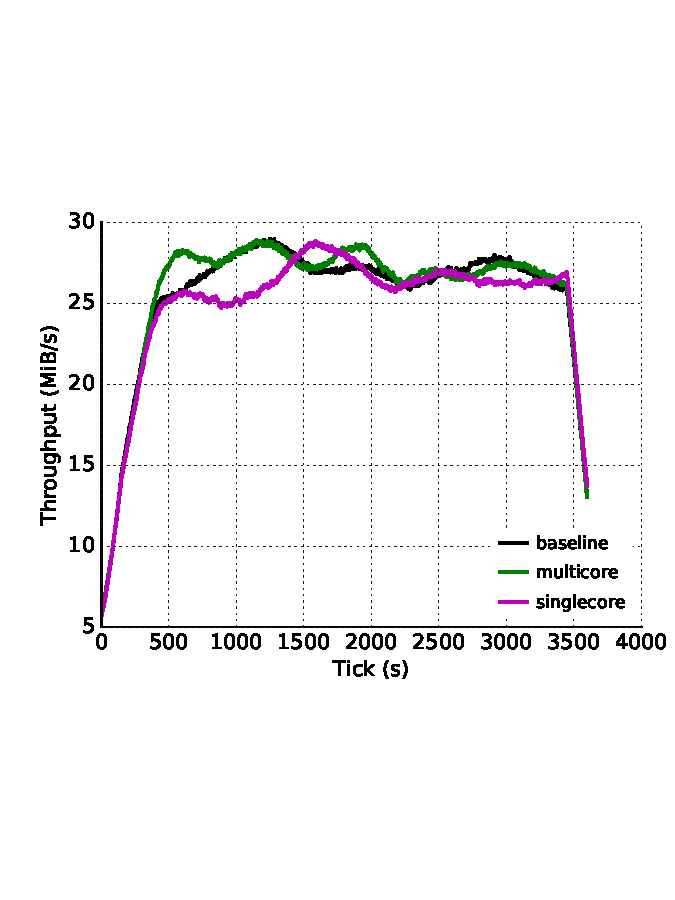
\includegraphics[trim={0 3cm 0 3cm}, clip, width=1.0\textwidth]{images/overhead_throughput.pdf}
		\caption{Throughput Overhead}
		\label{fig:overhead_throughput}
	\end{subfigure}
	\begin{subfigure}[t]{0.32\textwidth} \centering
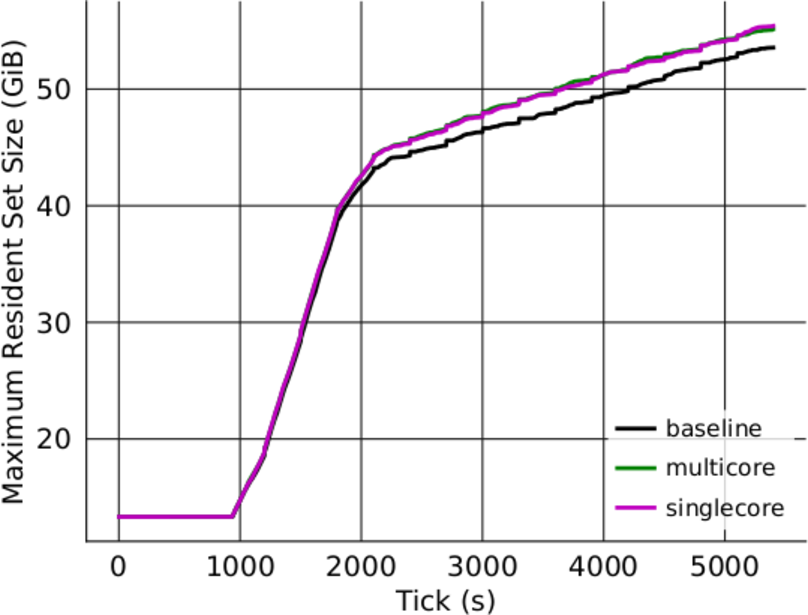
\includegraphics[trim={0 3cm 0 3cm}, clip, width=1.0\textwidth]{images/overhead_memory.pdf}
		\caption{Simulation Memory}
		\label{fig:overhead_shadow}
	\end{subfigure}
	\caption{Global Overhead --- Comparison of overhead in pure multicore
          and singlecore network
          conditions. Figure~\ref{fig:overhead_ttlastbyte} shows two sets of
          download time CDF curves for each file size (2 MiB and 5 MiB),
          Figure~\ref{fig:overhead_throughput} shoes the 5 minute moving average
          throughput over time, and Figure~\ref{fig:overhead_shadow} shows the
          memory consumption across the experiment lifetime. The simulation
          includes 100 relays, 2 authorities, 1 ledger authority, 10
          intermediaries and 1000 Tor clients scaled down from the public
          consensus file `2018-02-03-00-00-00-consensus'.}
	\label{fig:overhead}
\end{figure*}

Our findings indicate that even in the worst case scenario, our system incurs
statistically negligible overhead at these scales across all three measures of
download time, throughput, and memory usage. This in line with the raw bandwidth
overhead observations in which a small fraction ($< 1\%$) of the network traffic
is attributable to moneTor payment messages. This is true for all of our trials
which feature a payment rate of 1 payment (1 cell) every 1000 data cells
exchanged in either direction. It is also possible to increase the payment rate
for more fairness if needed, as long as the total overhead induced from control
cells is kept under an acceptable fraction of the overall data bandwidth. 
%%%
% Reading this sentence appears to be unclear to me
%%%
%This
%low overhead cost is separate from adverse networking effects of prioritization,
%which has the potential to more drastically affect performance.

%\begin{table}
%  \caption[Overhead Throughput Total]{\textbf{Overhead Throughput Total} Total
%    transferred application traffic over the duration of the over head trials
%    compared to total transferred payment traffic.}
%  \begin{center}
%    \begin{tabular}{ c c c }
%      & Throughput (GiB) & Payment Traffic (GiB) \\ \hline
%      Baseline & 128.4 & 0.000 \\
%      Multi-Core & 129.1 & 0.449 \\
%      Single-Core & 127.6 & 0.396
%    \end{tabular}
%  \end{center}
%  \label{tab:overhead}
%\end{table}

\subsubsection{Payment Latency}

Given results from our data collection, we surmise that payment latency is a
crucial factor in servicing our front-loaded clients. To this end, we measure
the distribution of completion times for various steps in the protocol. The
results shown here are collected from a worst case multicore experiment
featuring 100 relays and 1000 clients all of whom run premium circuits. To
highlight the effects of native latency in the Tor network, we show payments
split across each relay role of guard, middle, and exit. Recall that moneTor
makes use of high-overhead, low-marginal cost payment channels. The bulk of the
cost in our scheme lies in the conduction of the nanopayment channel
\emph{establish} and \emph{close} protocols as shown in
Figure~\ref{fig:payments_establish} and Figure~\ref{fig:payments_close}. Notice
that close operations are about twice as time consuming as establish operations
reflecting the need for the relay to close his half of the nanopayment channel
before the client can complete hers. Figure~\ref{fig:ttfp} illustrates time to
first payment, our most revealing latency metric. This measure includes the
overhead in channel establishment when we do not have available preemptive
channels. In the best case scenario, when all three payment channels have been
correctly pre-built for the circuit, this measure is equivalent to a single trip
toward each relay. Comparing this Figure~\ref{fig:ttfp} to
Figure~\ref{fig:payments_establish}, we observe the effectiveness of preemptive
channel building.

\begin{figure*} \centering
	\begin{subfigure}[t]{0.32\textwidth} \centering
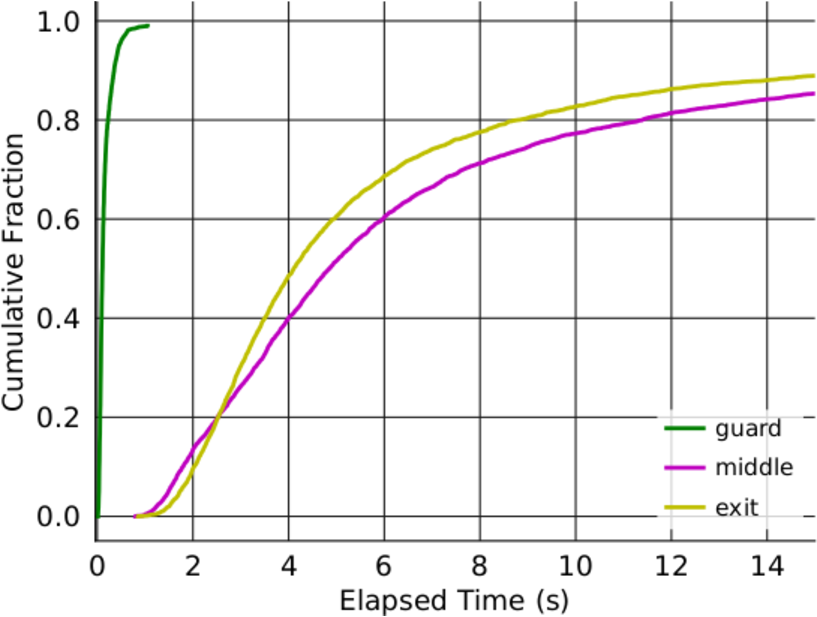
\includegraphics[trim={0 3cm 0 3cm}, clip, width=1.0\textwidth]{images/payment_establish.pdf}
		\caption{Nano-Establish}
\label{fig:payments_establish}
	\end{subfigure}
	\begin{subfigure}[t]{0.32\textwidth} \centering
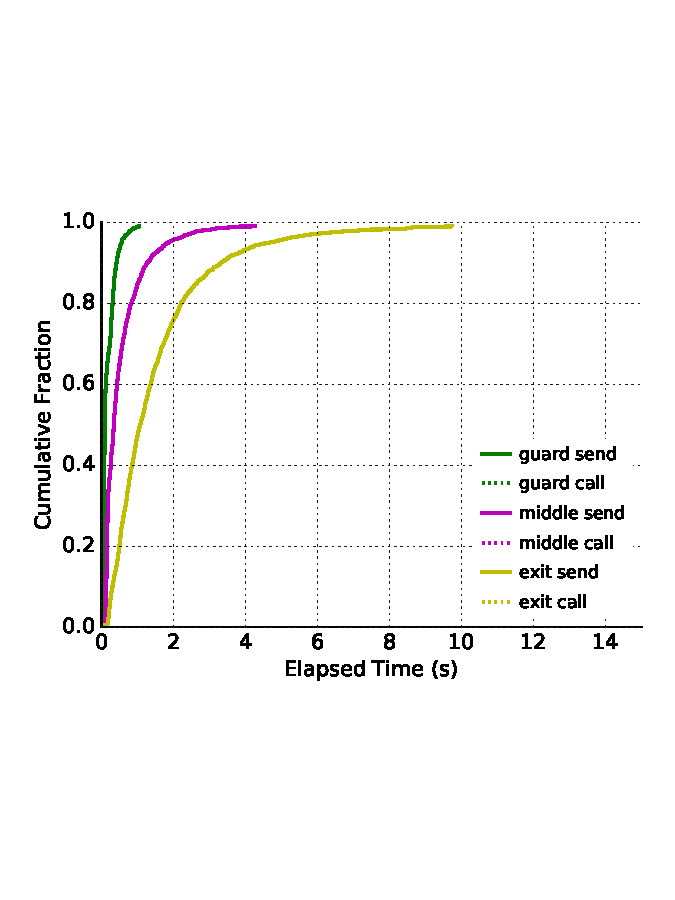
\includegraphics[trim={0 3cm 0 3cm}, clip, width=1.0\textwidth]{images/payment_pay.pdf}
		\caption{First Payment}
\label{fig:ttfp}
	\end{subfigure}
	\begin{subfigure}[t]{0.32\textwidth} \centering
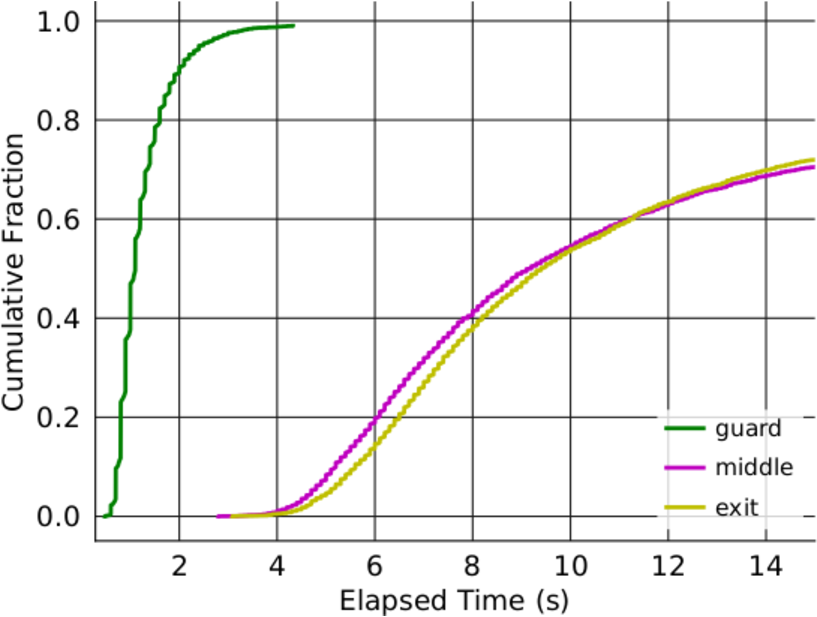
\includegraphics[trim={0 3cm 0 3cm}, clip, width=1.0\textwidth]{images/payment_close.pdf}
		\caption{Nano-Close}
\label{fig:payments_close}
	\end{subfigure}
	\caption{Protocol Execution Time --- Time to finish each protocol step
          split across interactions with each of the three relay. The simulation
          includes 100 relays, 2 authorities, 1 ledger authority, 10
          intermediaries and 1000 Tor clients scaled down from the public
          consensus file `2018-02-03-00-00-00-consensus'.}
\label{fig:latencymeasurements}
\end{figure*}

In all protocol phases, we observe that latency for guard relays are negligible
in comparison to the middle and exit relays, further validating our design
decision to implement special directly paid guard channels.

\subsubsection{Network Priority}
\label{sec:priority_exp}

Our final set of experiments studies the success of our scheme in delivering
prioritized traffic for premium users. To perform this analysis, we prepared
sets of three small experiments with varying modifier priorities
$\alpha \in \{0, 0.25, 0.5\}$, where $\alpha = 0$ represents the baseline
control. Our first set of experiments assuming 50\% of premium users is shown in
Figures \ref{fig:modifier_pr50_web}, \ref{fig:modifier_pr50_bulk}, and
\ref{fig:modifier_pr50_all}. From this illustration, is it evident that premium
users enjoy an advantage in internet speed compared to nonpremium users and that
this advantage is more pronounced with the higher priority modifier. Moreover,
the evenly split premium and nonpremium performance ``averages out'' to
approximately mirror the baseline experiment, indicating little loss in overall
network performance, and confirming our overhead experiment.

A more realistic model should most likely assume a smaller minority of premium
users. We therefore conducted a separate set of experiments to study an
environment comprised of only 25\% premium users who, according to
Equation~\ref{eq:flow}, should expect an even greater benefit on a per-user
basis. Figures \ref{fig:modifier_pr25_web}, \ref{fig:modifier_pr25_bulk}, and
\ref{fig:modifier_pr25_all} shows that this is indeed the result. Users across
the spectrum of web speed enjoyed $\approx 100\%$ improvements in download
speeds relative to nonpremium users --- likely enough to induce some amount of
monetary exchange. 


\begin{figure*} \centering
	\begin{subfigure}[t]{0.32\textwidth} \centering
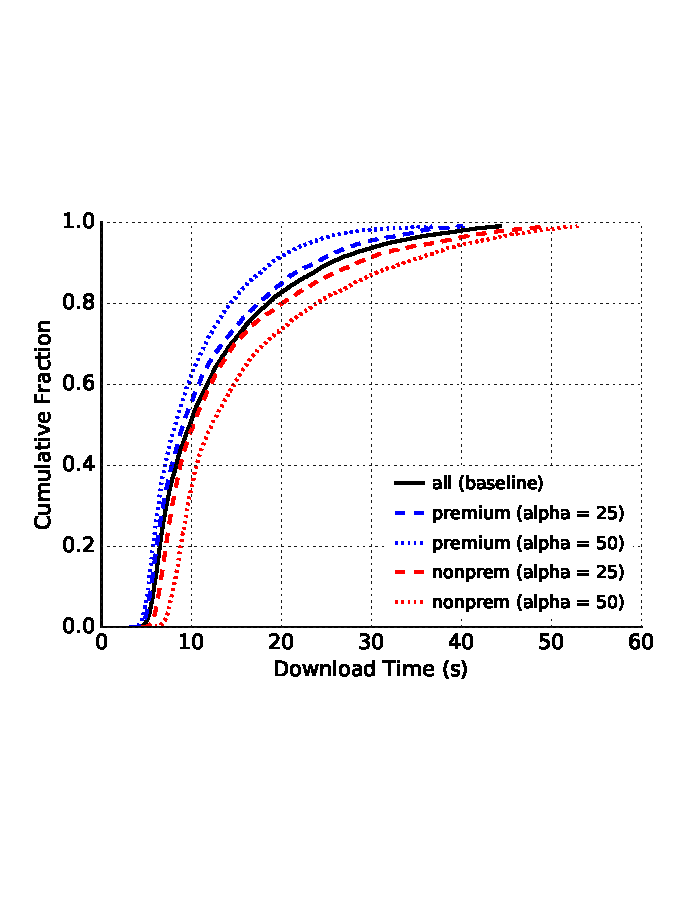
\includegraphics[trim={0 3cm 0 3cm}, clip, width=1.0\textwidth]{images/modifier_pr50_web.pdf}
		\caption{Web Download Time}
\label{fig:modifier_pr50_web}
	\end{subfigure}
	\begin{subfigure}[t]{0.32\textwidth} \centering
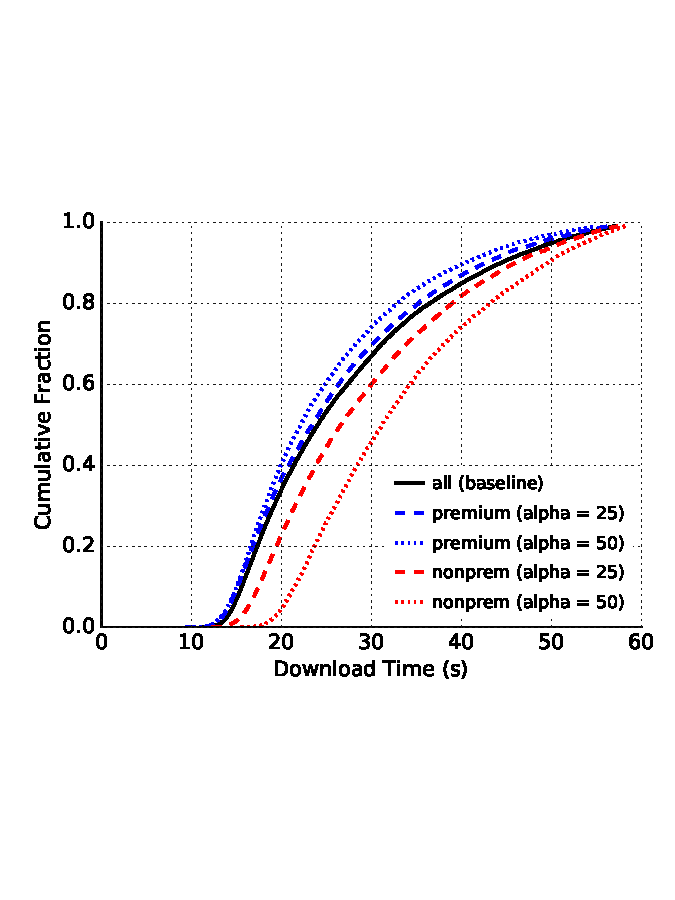
\includegraphics[trim={0 3cm 0 3cm}, clip, width=1.0\textwidth]{images/modifier_pr50_bulk.pdf}
		\caption{Bulk Download Time}
\label{fig:modifier_pr50_bulk}
	\end{subfigure}
	\begin{subfigure}[t]{0.32\textwidth} \centering
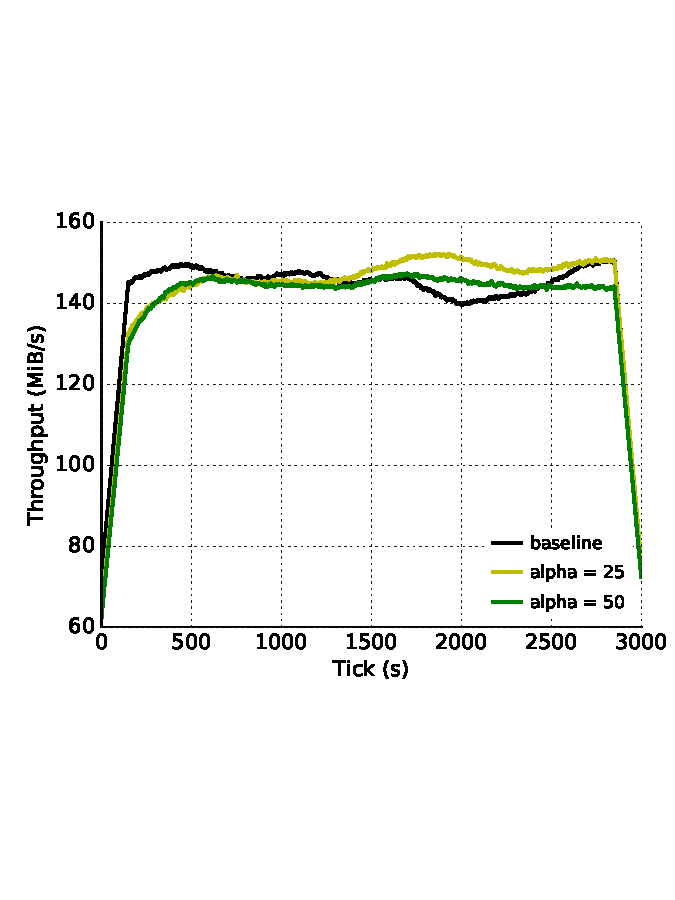
\includegraphics[trim={0 3cm 0 3cm}, clip, width=1.0\textwidth]{images/modifier_pr50_all.pdf}
		\caption{Throughput}
\label{fig:modifier_pr50_all}
	\end{subfigure}
	\begin{subfigure}[t]{0.32\textwidth} \centering
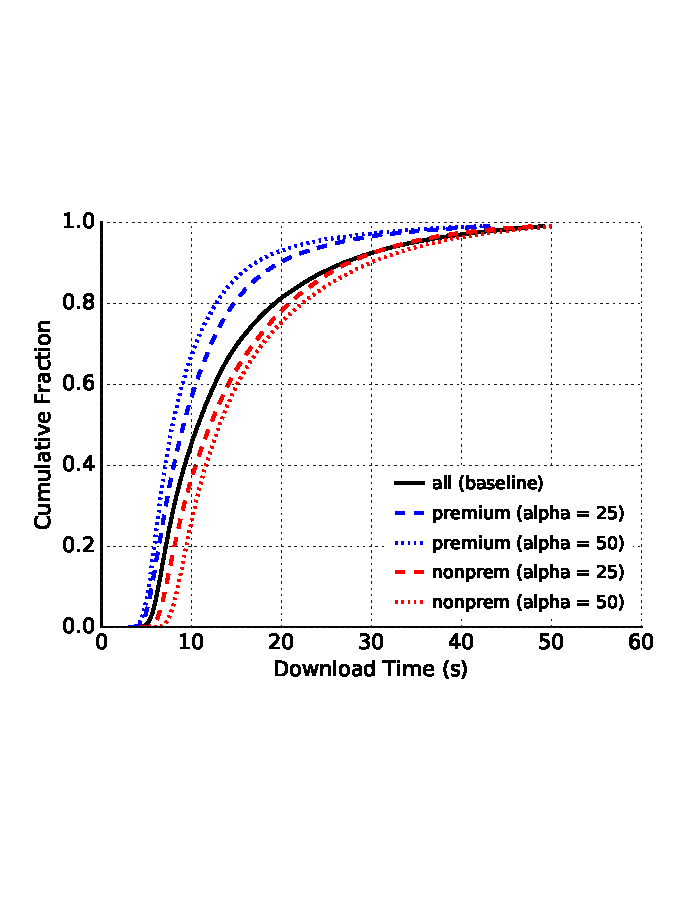
\includegraphics[trim={0 3cm 0 3cm}, clip, width=1.0\textwidth]{images/modifier_pr25_web.pdf}
		\caption{Web Download Time}
\label{fig:modifier_pr25_web}
	\end{subfigure}
	\begin{subfigure}[t]{0.32\textwidth} \centering
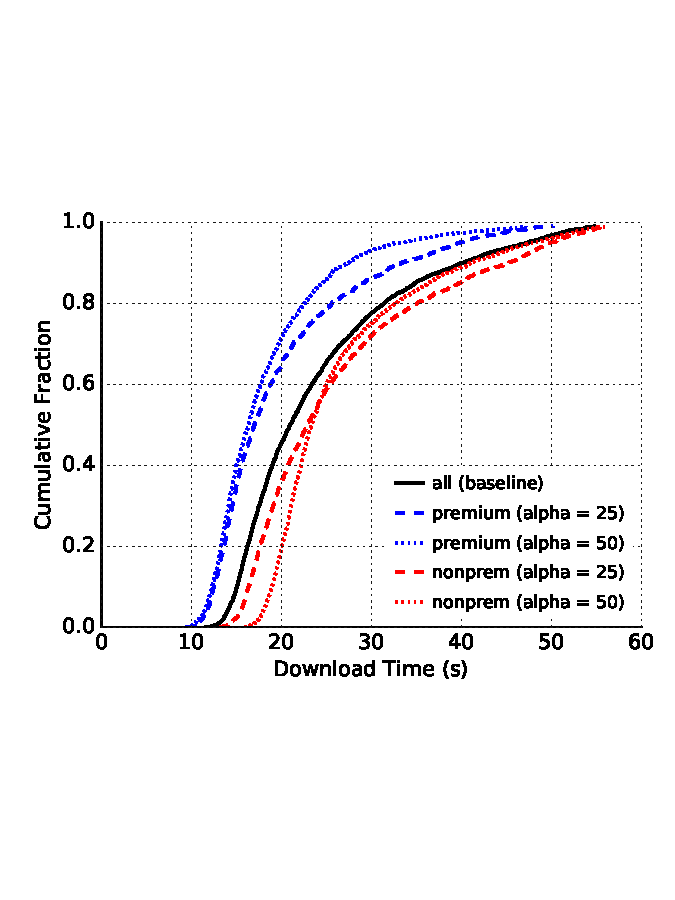
\includegraphics[trim={0 3cm 0 3cm}, clip, width=1.0\textwidth]{images/modifier_pr25_bulk.pdf}
		\caption{Bulk Download Time}
\label{fig:modifier_pr25_bulk}
	\end{subfigure}
	\begin{subfigure}[t]{0.32\textwidth} \centering
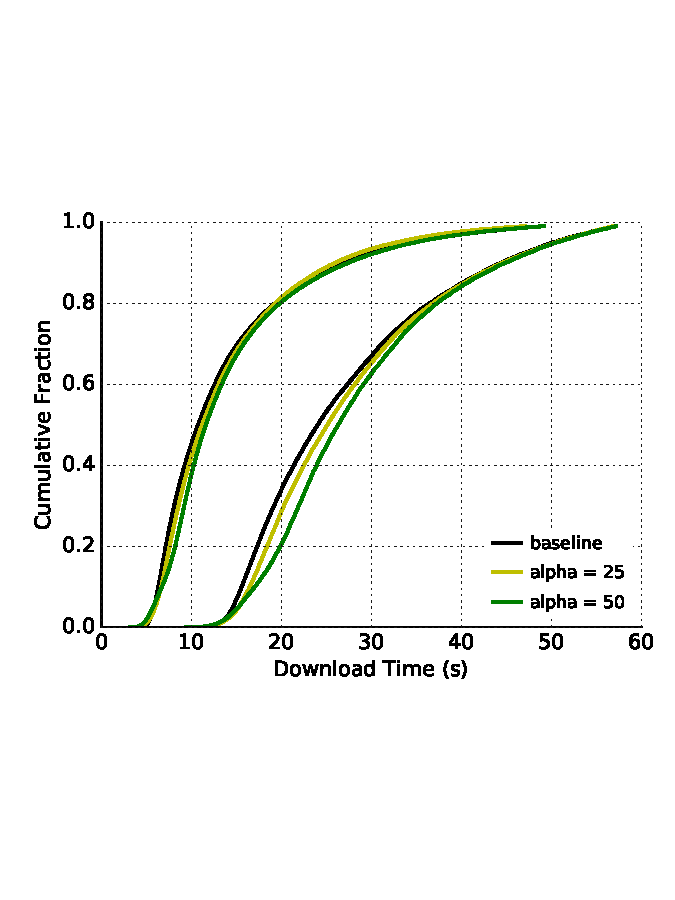
\includegraphics[trim={0 3cm 0 3cm}, clip, width=1.0\textwidth]{images/modifier_pr25_all.pdf}
		\caption{Throughput}
\label{fig:modifier_pr25_all}
	\end{subfigure}
	\caption{Prioritization Benefit --- Performance differentiation between
          paid and unpaid users. The first row displays results with 50\%
          premium users while the second row displays results for 25\% premium
          users. Simulations feature 250 relays, 2 authorities, 1 ledger
          authority, 25 intermediaries and 2500 Tor clients scaled down from the
          public consensus file `2018-02-03-00-00-00-consensus'.}
\label{fig:modifier}
\end{figure*}

%\begin{table}
%  \caption[Prioritized Throughput]{\textbf{Prioritized Throughput} Tabulate total
%    number of successful file transfers and timeout errors across varying levels
%    of prioritization}
%  \begin{center}
%    \begin{tabular}{ c c c c}
%      & Throughput & Timeouts & Timeout \\
%      & (GiB) & (Web) & (Bulk) \\ \hline
%      $\alpha = 0.00$ & 427 & 115 & 354 \\ \hline
%      $\alpha = 0.25,\ pr\% = 50$ & 429 & 206 & 404 \\
%      $\alpha = 0.25,\ pr\% = 25$ & 433 & 231 & 459 \\ \hline
%      $\alpha = 0.50,\ pr\% = 50$ & 420 & 233 & 356 \\
%      $\alpha = 0.50,\ pr\% = 25$ & 414 & 381 & 513 \\
%    \end{tabular}
%  \end{center}
%  \label{tab:modifier}
%\end{table}

%%% Local Variables:
%%% mode: latex
%%% TeX-master: "../main"
%%% End:



\section{Limitations}
\label{sec:limitations}

\section{Code and Data Reproducibility}
\label{sec:code}

\section{Conclusion}
\label{sec:conclusion}
\bibliographystyle{ACM-Reference-Format}
\bibliography{ccs-sample}

\end{document}
